\documentclass[a4paper]{article}

\usepackage[fontset=fandol]{ctex}
\usepackage{amsmath, amssymb}
\usepackage{graphicx}
\usepackage[margin=2.2cm]{geometry}
\usepackage[most]{tcolorbox}
\usepackage{etoolbox}
\usepackage{listings}
\usepackage{hyperref}
\usepackage{xurl}
\usepackage{booktabs}
\usepackage{longtable}
\usepackage{tabularx}
\usepackage{array}
\usepackage{subcaption}
\usepackage{float}
\usepackage{enumitem}
\usepackage{tikz}
\usepackage{multirow}

\hypersetup{
    colorlinks=true,
    linkcolor=blue!50!black,
    urlcolor=blue!60!black,
    citecolor=blue!50!black
}

\newtcolorbox{findingbox}[1]{
    enhanced,
    colback=green!5!white,
    colframe=green!45!black,
    colbacktitle=green!45!black,
    coltitle=white,
    fonttitle=\bfseries,
    title=#1,
    sharp corners
}

\newtcolorbox{evidencebox}[1]{
    enhanced,
    colback=blue!4!white,
    colframe=blue!65!black,
    colbacktitle=blue!65!black,
    coltitle=white,
    fonttitle=\bfseries,
    title=#1,
    sharp corners
}

\newtcolorbox{riskbox}[1]{
    enhanced,
    colback=red!4!white,
    colframe=red!70!black,
    colbacktitle=red!70!black,
    coltitle=white,
    fonttitle=\bfseries,
    title=#1,
    sharp corners
}

\newtcolorbox{methodbox}[1]{
    enhanced,
    colback=yellow!9!white,
    colframe=yellow!60!black,
    colbacktitle=yellow!60!black,
    coltitle=black,
    fonttitle=\bfseries,
    title=#1,
    sharp corners
}

\newcolumntype{Y}{>{\raggedright\arraybackslash}X}
\setlist[itemize]{leftmargin=1.8em}
\newcommand{\filepath}[1]{\nolinkurl{#1}}

\newcommand{\reporttitle}{CCH Client Abort GUI 改动部署核查报告}
\newcommand{\reportsubtitle}{日志页与 Availability 页的可见变化、代码映射与运维含义}
\newcommand{\reportauthors}{Codex}
\newcommand{\reportdate}{2026-03-25}
\newcommand{\researchquestion}{重新部署 \filepath{classify-client-abort-observability} 之后，GUI 具体改了哪里，这些改动分别落在哪些页面、组件和数据链路上？}
\newcommand{\reportscope}{仓库 \filepath{/home/fanghaotian/Desktop/src/cch/claude-code-hub}，live 实例 \url{http://127.0.0.1:23000}，证据截止到 2026-03-25 15:16 CST。}
\newcommand{\reportaudience}{claude-code-hub 维护者、运维排障者、需要向团队解释 499 语义的人}
\newcommand{\sourcewindow}{代码、数据库、浏览器截图、admin backfill 执行结果，访问日期均为 2026-03-25}
\newcommand{\reportcoverpath}{figures/logs-session-continued-page.png}

\begin{document}

\begin{titlepage}
\centering
{\Large 深度研究报告\par}
\vspace{1.0cm}
{\huge\bfseries \reporttitle\par}
\vspace{0.5cm}
{\Large \reportsubtitle\par}
\vspace{0.9cm}
{\large \reportauthors\par}
\vspace{0.2cm}
{\large \reportdate\par}
\vspace{1.0cm}
\includegraphics[width=0.84\textwidth,height=0.42\textheight,keepaspectratio]{\reportcoverpath}\par

\vfill
\begin{tcolorbox}[width=0.94\textwidth, colback=black!2!white, colframe=black!60, sharp corners]
\textbf{核心问题}：\researchquestion\par
\textbf{研究范围}：\reportscope\par
\textbf{目标读者}：\reportaudience\par
\textbf{证据窗口}：\sourcewindow\par
\end{tcolorbox}
\end{titlepage}

\tableofcontents
\newpage

\section{执行摘要}

\begin{findingbox}{核心结论}
这次 GUI 改动主要落在两个界面：\textbf{日志页}和\textbf{Availability 页}。前者新增了 \filepath{clientAbortOutcome} 维度的筛选、列表内联 badge、以及详情抽屉里的“客户端中断分类”信息块；后者则新增了本地 client abort 的专属 counters 卡片，并把这类请求从 provider availability 失败统计中剥离出去。
\end{findingbox}

更具体地说：

\begin{itemize}
\item 访问入口虽然仍保留 \filepath{/dashboard/logs} 和 \filepath{/dashboard/availability}，但 live GUI 实际会被重定向到 \filepath{/console/traffic/logs} 与 \filepath{/console/overview/availability}。
\item 这次改动既有\textbf{肉眼可见的新 UI 元素}，也有\textbf{已有 KPI 的语义修正}。后一类变化不一定新增一个按钮或模块，但会直接改变管理员对“499 是否意味着供应商失败”的理解。
\item 重新部署并执行 admin backfill 后，最近 7 天的 live 数据里已经能看到 \texttt{1451} 条 \texttt{after\_stream\_start}、\texttt{272} 条 \texttt{session\_continued}、\texttt{145} 条 long-running，因此新界面不是空壳，而是已经有稳定样本可展示。
\end{itemize}

\section{研究范围与方法}

\begin{methodbox}{研究方法}
本次说明文档基于四类证据：
\begin{itemize}
\item 仓库源码：用于定位 GUI 组件、数据查询、路由映射、数据库字段与回填接口。
\item live 页面截图：用于证明“用户现在实际能看到什么”。
\item 本地部署观测：用于确认 redeploy 已成功，实例处于健康状态。
\item 数据库统计：用于解释为什么某些新模块已经有内容，以及某些分类暂时为空。
\end{itemize}
\end{methodbox}

\subsection{部署与验证边界}

本次检查基于本机 live 实例 \url{http://127.0.0.1:23000}。健康检查在 2026-03-25 15:16 CST 返回 \texttt{\{"status":"ok"\}}，说明当前截图和数据库读取针对的是已经成功启动的新版本，而不是旧页面缓存。

\subsection{证据采集方式}

\begin{itemize}
\item 代码证据：直接读取 repo 当前工作树中的实现文件。
\item GUI 证据：登录 admin 后抓取 live 页面截图，截图元数据记录在 \filepath{capture-metadata.json}。
\item 历史数据补齐：通过 admin-only 路由 \filepath{/api/admin/client-abort-observability/backfill} 连续执行，直到 \texttt{hasMore=false}。
\item SQL 观测：在 live PostgreSQL 中统计最近 7 天 \texttt{499 CLIENT\_ABORTED} 的 outcome 分布。
\end{itemize}

\section{改动总表}

\begin{longtable}{p{2.2cm}p{3.2cm}p{4.6cm}p{4.4cm}}
\toprule
页面 / 区域 & 具体位置 & 用户可见变化 & 对应代码锚点 \\
\midrule
\endfirsthead
\toprule
页面 / 区域 & 具体位置 & 用户可见变化 & 对应代码锚点 \\
\midrule
\endhead
日志页 & 筛选面板的状态区 & 新增“客户端中断分类”下拉框，可选 \texttt{session\_continued}、\texttt{after\_stream\_start}、\texttt{before\_stream\_start} & \filepath{src/app/[locale]/dashboard/logs/_components/filters/status-filters.tsx:57-60,114-135} \\
日志页 & Active filters 区域与 URL & 新增 chip 展示，URL 支持 \filepath{clientAbortOutcome=} 参数，前后端都能保留筛选状态 & \filepath{active-filters-display.tsx:135-140}；\filepath{logs-query.ts:43-52,109-111}；\filepath{usage-logs-view-virtualized.tsx:165-179} \\
日志页 & 列表状态列 & 499 样本会在详情按钮旁显示一枚 outcome badge，例如“会话继续” & \filepath{virtualized-logs-table.tsx:824-848} \\
日志页 & 请求详情抽屉的 Summary Tab & 新增“客户端中断分类”信息块，显示 outcome、是否已开始流式输出、是否 long-running，以及 continuation request id / time & \filepath{SummaryTab.tsx:99-110,316-355}；\filepath{types.ts:64-71} \\
Availability 页 & overview 顶部概览 & 新增“客户端中断”统计卡片，展示 total / session continued / after stream start / before stream start / long-running & \filepath{overview-section.tsx:170-210}；\filepath{availability-dashboard.tsx:98-122} \\
Availability 页 & availability / error rate 计算语义 & 本地 \texttt{499 CLIENT\_ABORTED} 不再算 provider red failure，而是单独计入 client abort counters & \filepath{availability-service.ts:33-51,292-305,402-426}；\filepath{types.ts:44-60,84-85,118-119} \\
数据层 & message\_request + backfill & GUI 所需字段已入库并有索引，历史记录通过 admin backfill 补齐 & \filepath{schema.ts:491-496,563-565}；\filepath{client-abort-observability.ts:66-89,104-131}；\filepath{backfill/route.ts:15-56} \\
\bottomrule
\end{longtable}

\section{日志页改动详解}

\subsection{入口路径已经迁移到 console 模块}

虽然仓库里仍保留 \filepath{src/app/[locale]/dashboard/logs/page.tsx}，但它本身不再渲染页面，而是直接调用 \filepath{redirectLegacyConsoleRoute} 做旧路由转发。代码上：

\begin{itemize}
\item \filepath{logs/page.tsx:14-18} 把旧路径 \filepath{/dashboard/logs} 交给重定向工具。
\item \filepath{legacy-route-redirect.ts:34-66} 负责在鉴权后跳到真正的 console 路由。
\item \filepath{runtime-route-map.ts:92-102} 明确声明 logs 的真实页面是 \filepath{/console/traffic/logs}。
\end{itemize}

这与 live 抓图结果一致：截图元数据中记录的地址是 \url{http://127.0.0.1:23000/zh-CN/console/traffic/logs?clientAbortOutcome=session_continued\&statusCode=499}。

\subsection{筛选面板新增了一整条 client abort 维度}

图 \ref{fig:logs-page} 展示了 redeploy 后日志页的整体布局。最重要的新入口在筛选面板里。

\begin{figure}[H]
\centering
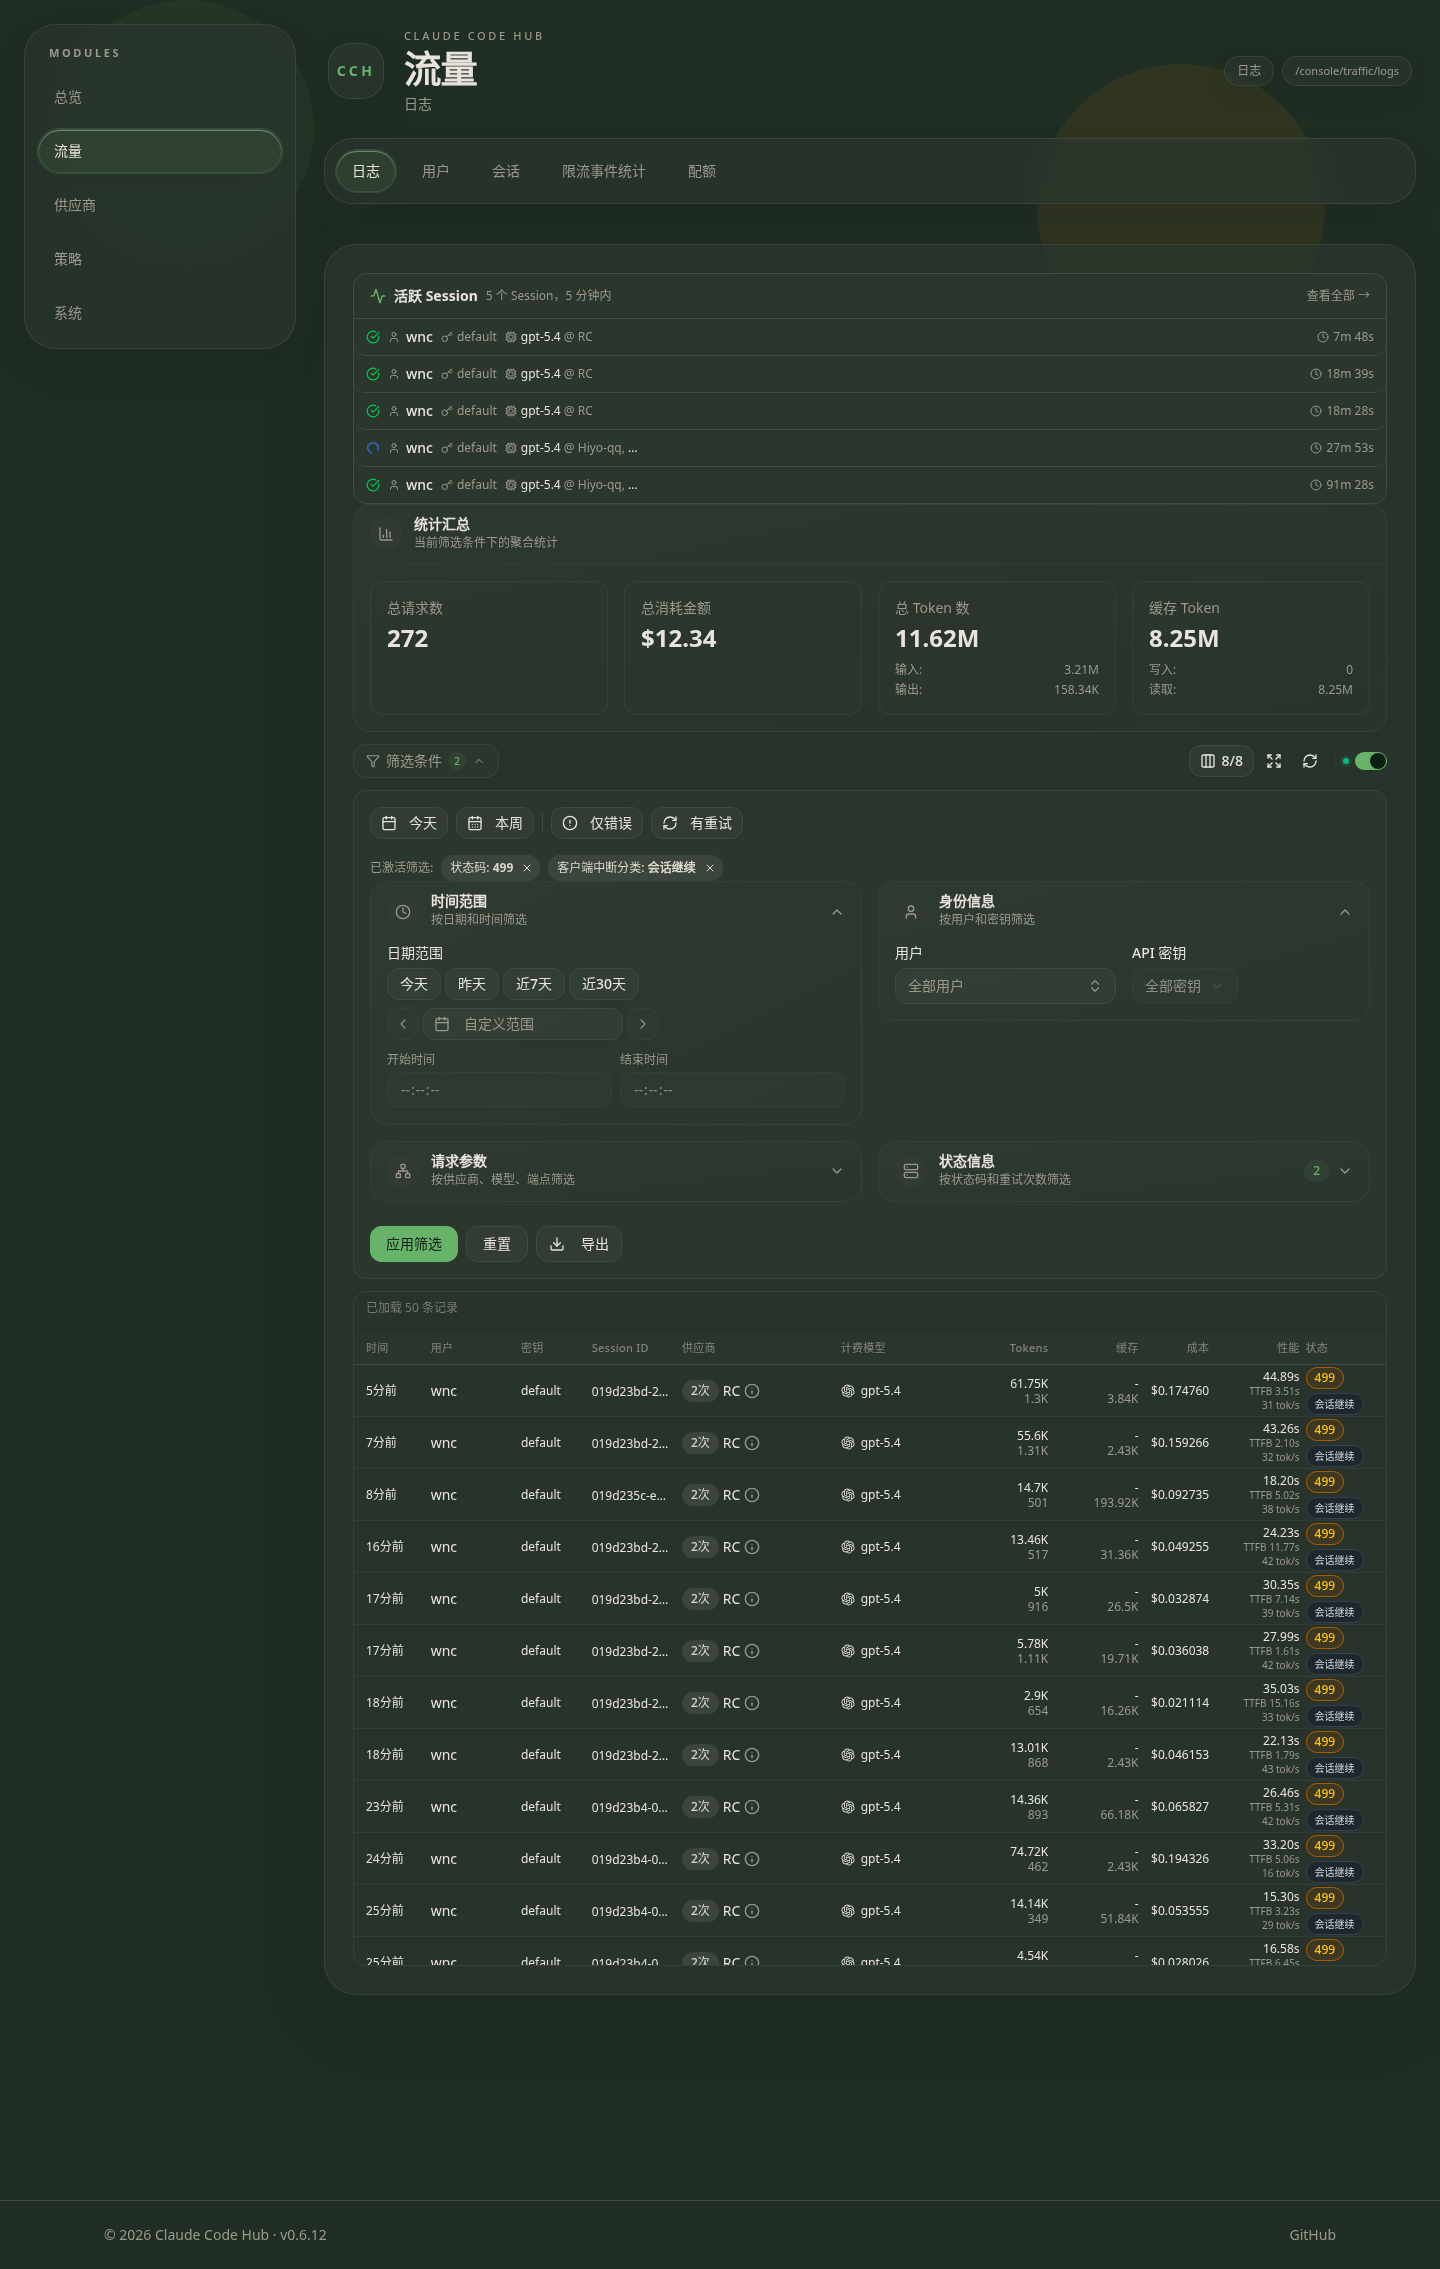
\includegraphics[width=0.74\textwidth]{figures/logs-session-continued-page.png}
\caption{日志页整体截图。来源：live GUI 截图，URL 为 \filepath{/zh-CN/console/traffic/logs?clientAbortOutcome=session_continued\&statusCode=499}。}
\label{fig:logs-page}
\end{figure}

从实现上看，这一层改动不是只加了一个下拉框，而是打通了四个环节：

\begin{itemize}
\item \filepath{status-filters.tsx:57-60} 在本地 filter state 中写入 \filepath{clientAbortOutcome}。
\item \filepath{status-filters.tsx:114-135} 渲染新的下拉选项和值映射。
\item \filepath{active-filters-display.tsx:135-140} 让已选 outcome 在筛选 chip 中以可读标签展示。
\item \filepath{logs-query.ts:43-52,109-111} 与 \filepath{usage-logs-view-virtualized.tsx:165-179} 让该字段进入 URL query，并在页面刷新或分享链接后可恢复。
\end{itemize}

后端配套也同步完成：\filepath{src/repository/_shared/usage-log-filters.ts:104-105} 会把该筛选转换成 \filepath{messageRequest.clientAbortOutcome = ...} 的 SQL 条件。因此这个控件并不是前端本地筛选，而是数据库级过滤。

\subsection{列表行本身增加了 outcome badge}

在日志列表里，用户点击“详情”之前就能看到一层更细粒度的 499 提示。对应实现是 \filepath{virtualized-logs-table.tsx:842-848}：如果某条日志存在 \filepath{log.clientAbortOutcome}，就额外渲染一枚灰色 outline badge，文本通过 \filepath{getClientAbortOutcomeLabelKey(...)} 走 i18n。

这意味着：

\begin{itemize}
\item 过去只能看到“499”这一层错误语义；
\item 现在可以在行级别直接区分“会话继续”和“流开始后中断”等情况。
\end{itemize}

\subsection{详情抽屉新增“客户端中断分类”区块}

这次日志页最实质的 GUI 改动在详情抽屉 Summary Tab。其渲染条件非常严格：

\begin{itemize}
\item \filepath{SummaryTab.tsx:99-103} 要求 \filepath{statusCode == 499} 且 \filepath{errorMessage == "CLIENT_ABORTED"}；
\item 同时必须已经有派生字段 \filepath{clientAbortOutcome}。
\end{itemize}

一旦条件满足，\filepath{SummaryTab.tsx:316-355} 会渲染三个层次的信息：

\begin{itemize}
\item outcome badge，例如“会话继续”或“已开始流式输出后中断”；
\item stream 状态 badge，由 \filepath{hasClientAbortStreamStarted(...)} 决定显示“已开始流式输出”还是“尚未开始流式输出”；
\item continuation 追踪字段，包括“由请求 \#... 继续”和 continuation 时间戳；
\item 如果请求时长超过阈值，还会显示 long-running badge。
\end{itemize}

图 \ref{fig:session-continued-panel} 和图 \ref{fig:after-stream-panel} 分别展示了 \texttt{session\_continued} 与 \texttt{after\_stream\_start} 两种 live 样例。

\begin{figure}[H]
\centering

\includegraphics[width=0.86\textwidth]{figures/client-abort-section-session-continued.png}
\caption{日志详情中的 \texttt{session\_continued} 样例。来源：live GUI 裁剪图，展示“会话继续”“已开始流式输出”“由请求 \#27783 继续”“继续时间 2026-03-25T06:59:06.295Z”。}
\label{fig:session-continued-panel}
\end{figure}

\begin{figure}[H]
\centering

\includegraphics[width=0.86\textwidth]{figures/client-abort-section-after-stream.png}
\caption{日志详情中的 \texttt{after\_stream\_start} 样例。来源：live GUI 裁剪图，展示“已开始流式输出后中断”“已开始流式输出”两枚 badge。}
\label{fig:after-stream-panel}
\end{figure}

为了让这个面板有数据，repository 和详情 props 也一起扩展了：

\begin{itemize}
\item \filepath{usage-logs.ts:207-210,260-263} 把四个 client abort 字段从数据库映射到行数据。
\item \filepath{error-details-dialog/types.ts:64-71} 把这些字段纳入 Summary Tab / Metadata Tab 共享 props。
\end{itemize}

\section{Availability 页改动详解}

\subsection{入口同样已迁移到 console overview}

Availability 页遵循与 logs 相同的 console 路由迁移模式：

\begin{itemize}
\item \filepath{availability/page.tsx:12-15} 重定向旧入口 \filepath{/dashboard/availability}。
\item \filepath{runtime-route-map.ts:80-90} 指向真实页面 \filepath{/console/overview/availability}。
\end{itemize}

因此，live 截图对应的页面 URL 是 \url{http://127.0.0.1:23000/zh-CN/console/overview/availability}。

\subsection{可见改动一：overview 顶部新增 client abort counters 卡片}

图 \ref{fig:availability-overview} 显示的是 redeploy 后 Availability 页面顶部区域。除了原有的 system availability、avg latency、error rate、active probes 四个 KPI 外，下面多出一块 “客户端中断”卡片。

\begin{figure}[H]
\centering
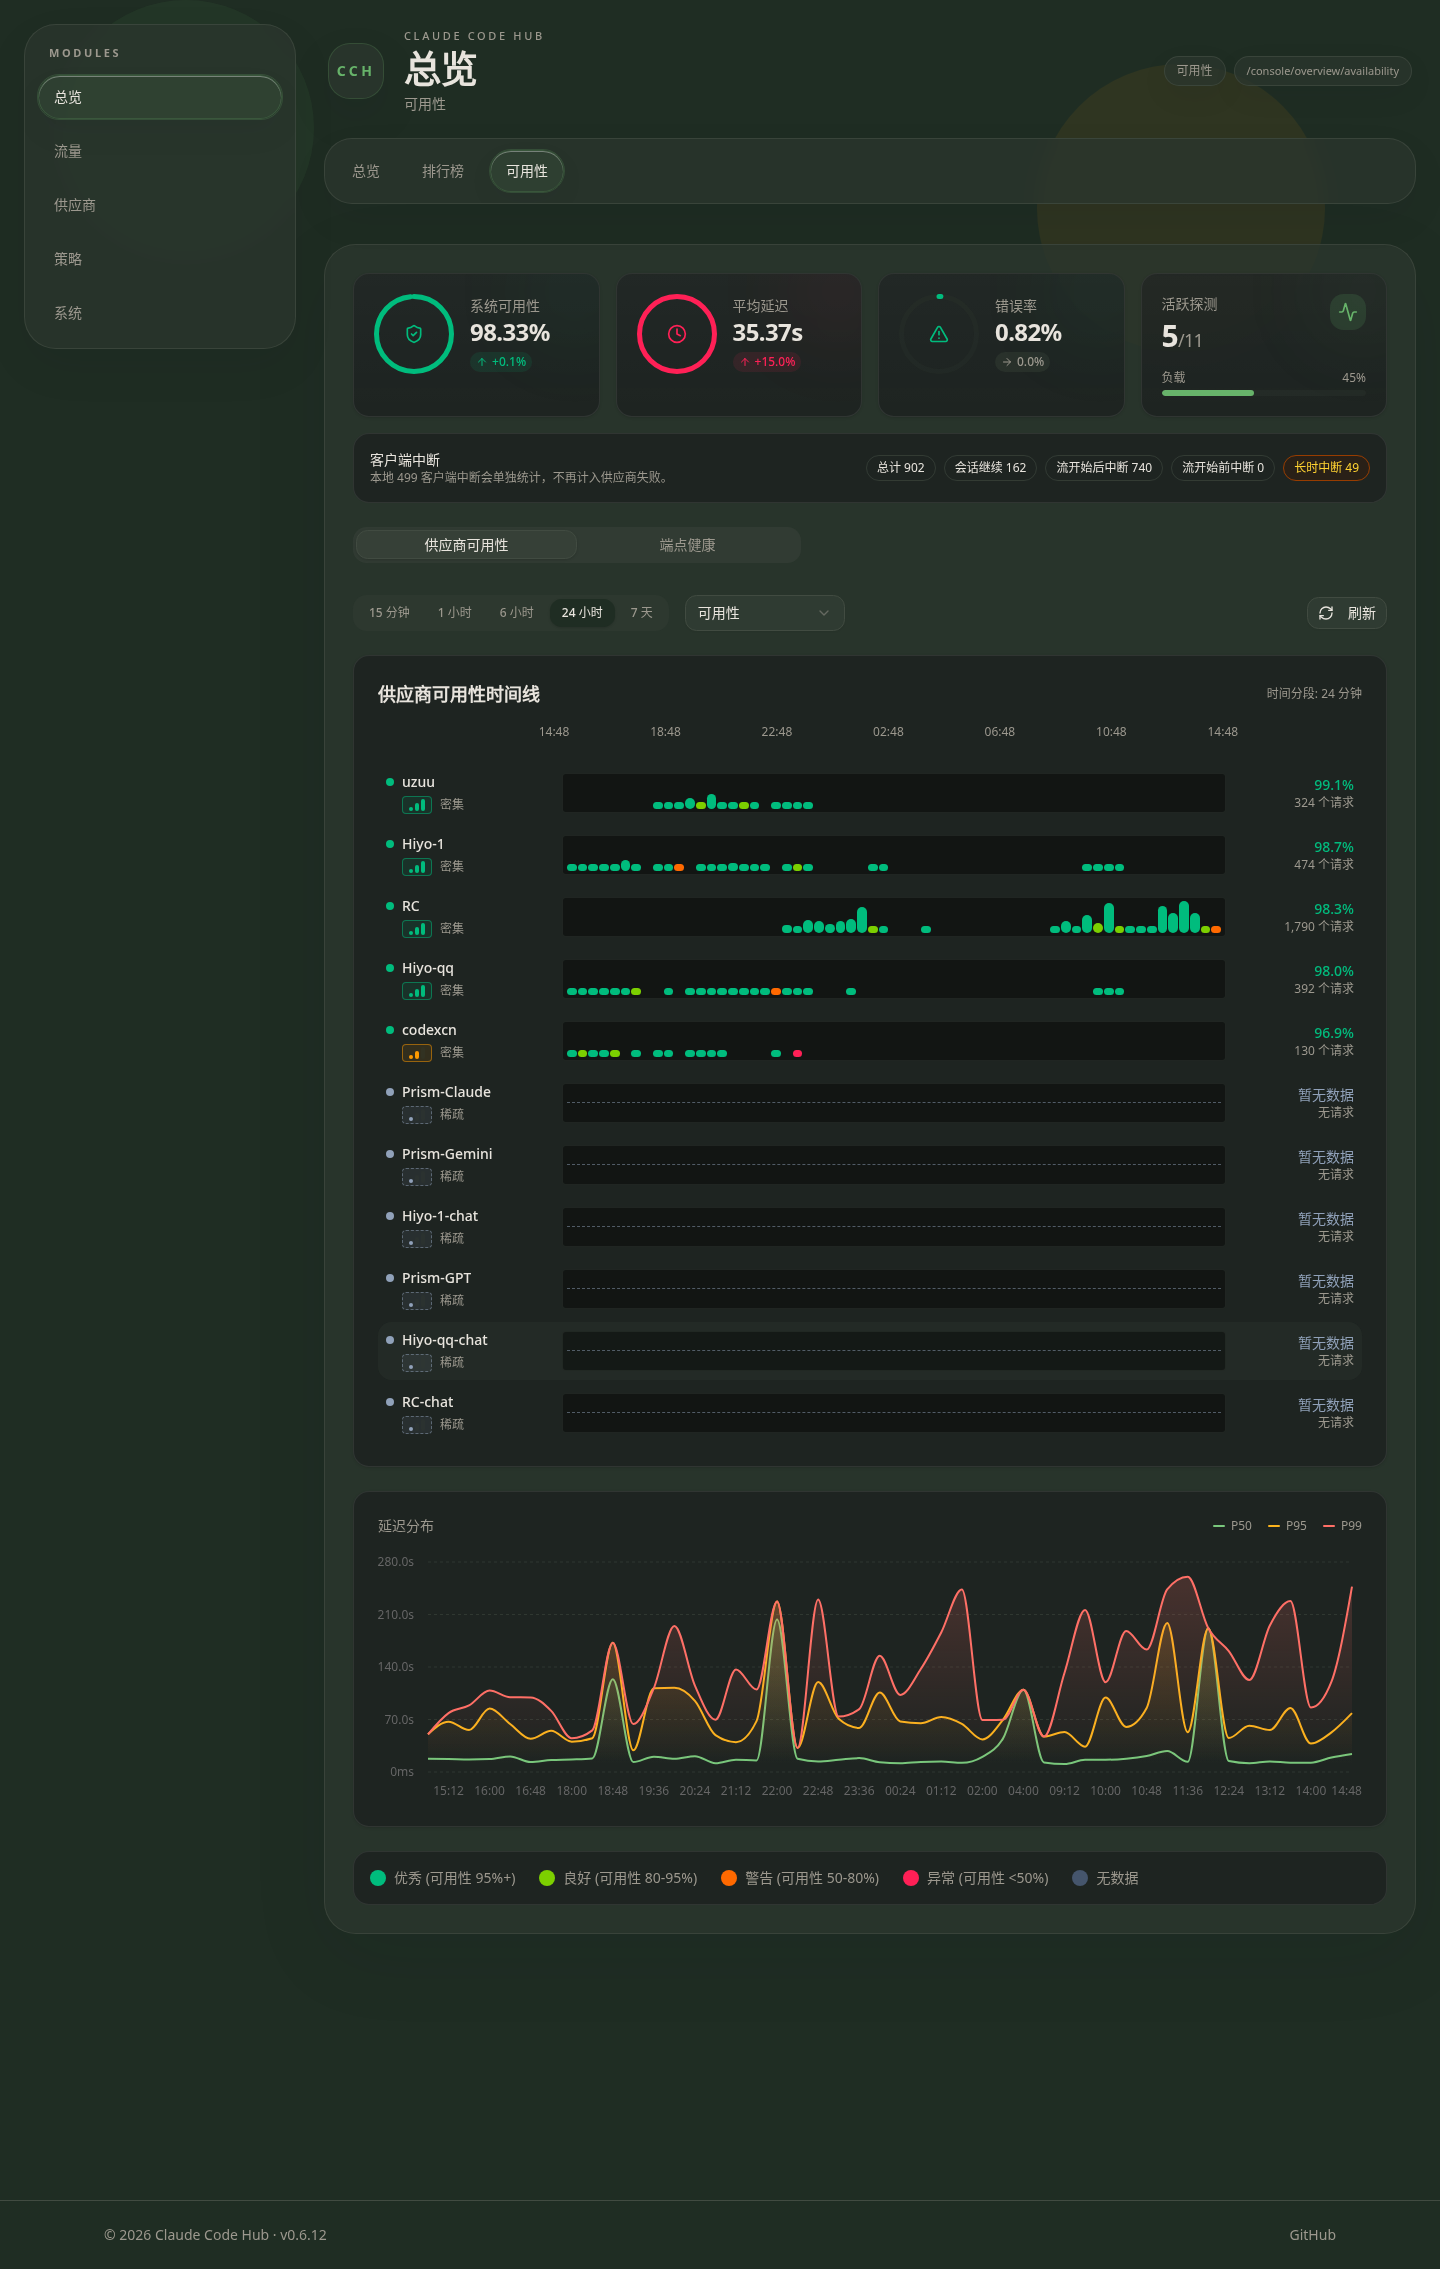
\includegraphics[width=0.82\textwidth]{figures/availability-overview.png}
\caption{Availability overview live 截图。来源：\filepath{/zh-CN/console/overview/availability} 页面截图。图中四个主 KPI 下方新增“客户端中断”统计带。}
\label{fig:availability-overview}
\end{figure}

从代码上，这个卡片由两层驱动：

\begin{itemize}
\item \filepath{availability-dashboard.tsx:98-122} 从 API 返回结果中提取 \filepath{clientAbortCounts} 并传给 overview。
\item \filepath{overview-section.tsx:170-210} 在 \filepath{clientAbortCounts.total > 0} 时渲染 counters 区块，包括 total、session continued、after stream start、before stream start、long-running 五个数。
\end{itemize}

\subsection{可见改动二：已有 KPI 的语义已经改变}

这一点比新增卡片更关键，因为它直接改变管理员如何解读错误率和可用性。

\begin{evidencebox}{语义变化的核心}
\filepath{availability-service.ts:41-50} 明确规定：如果一条请求同时满足“本地 client abort 派生 outcome 已存在”和“状态是本地 \texttt{499 CLIENT\_ABORTED}”，那么这条请求会被分类为 \texttt{unknown}，\textbf{不计入 availability 的 green/red 分母}，但会\textbf{计入 client abort counters}。
\end{evidencebox}

对应公式可以写成：

$$
\text{availability} = \frac{G}{G + R}
$$

\begin{itemize}
\item $G$：计入 availability 的绿色请求数量
\item $R$：计入 availability 的红色请求数量
\item 本地 \texttt{499 CLIENT\_ABORTED}：不进入 $G$，也不进入 $R$，只进入独立的 client abort 计数
\end{itemize}

这套规则在代码里的落点是：

\begin{itemize}
\item \filepath{availability-service.ts:33-86} 定义单条请求的分类规则。
\item \filepath{availability-service.ts:292-305} 在 time bucket 聚合时分别累加 red/green 与 client abort counters。
\item \filepath{availability-service.ts:402-426} 计算系统级 aggregation，并返回全局 \filepath{clientAbortCounts}。
\item \filepath{types.ts:54-60,73-95,149-163} 把这些计数显式纳入 availability 返回类型。
\end{itemize}

因此，Availability 页有两种层面的变化：

\begin{itemize}
\item 一种是肉眼能看到的 counters 卡片；
\item 另一种是肉眼不一定会立刻意识到，但会改变数值解释的 KPI 去偏：本地 client abort 不再被误读成 provider failure。
\end{itemize}

\section{GUI 背后的数据前提}

\subsection{数据库已经具备专门字段与索引}

这次 GUI 之所以能显示 continuation request id、long-running badge 等细节，不是靠前端即时推断，而是因为 \filepath{message\_request} 已经扩展了专门字段：

\begin{itemize}
\item \filepath{schema.ts:491-496} 新增 \filepath{client_abort_outcome}、\filepath{client_abort_long_running}、\filepath{client_abort_continued_by_request_id}、\filepath{client_abort_continued_at}。
\item \filepath{schema.ts:563-565} 新增 \filepath{client_abort_outcome} 活跃索引，保证 logs filter 可走数据库索引。
\end{itemize}

\subsection{分类与 continuation 规则是稳定函数，不是页面猜测}

\filepath{src/lib/client-abort-observability.ts} 定义了这套派生规则：

\begin{itemize}
\item \filepath{47-57}：如何判断“流是否已经开始”；
\item \filepath{66-89}：如何得到 provisional outcome 与 long-running 标记；
\item \filepath{104-131}：如何判断后续请求是否在 continuation window 内，从而把 outcome 升级为 \texttt{session\_continued}。
\end{itemize}

\subsection{历史数据通过 admin backfill 补齐}

GUI 新模块之所以在 redeploy 后马上有内容，是因为历史 499 也被补齐了：

\begin{itemize}
\item \filepath{backfill/route.ts:15-56} 提供 admin-only 回填接口；
\item 本次执行直到 \texttt{hasMore=false}；
\item 当前最近 7 天 live 数据中，\texttt{after\_stream\_start = 1451}，\texttt{session\_continued = 272}，\texttt{long-running = 145}。
\end{itemize}

\begin{table}[H]
\centering
\begin{tabular}{lr}
\toprule
分类 & 最近 7 天条数 \\
\midrule
\texttt{after\_stream\_start} & 1451 \\
\texttt{session\_continued} & 272 \\
\texttt{before\_stream\_start} & 0 \\
\texttt{long-running} & 145 \\
\bottomrule
\end{tabular}
\caption{live 数据库中的 client abort 派生结果统计。来源：\filepath{live-observations.md}。}
\end{table}

这张表解释了一个重要事实：\texttt{before\_stream\_start} 目前不是“没做”，而是“代码支持，但当前 7 天窗口里没有样本落到这一类”。

\section{文案与多语言改动位置}

新的 GUI 文案没有硬编码在组件里，而是进入了 dashboard i18n 资源。以中文包为例：

\begin{itemize}
\item \filepath{messages/zh-CN/dashboard.json:120-128} 定义筛选器文案与 outcome 标签。
\item \filepath{messages/zh-CN/dashboard.json:224-229} 定义 logs 表格/行级 badge 对应的 outcome 标签。
\item \filepath{messages/zh-CN/dashboard.json:259-265} 定义详情抽屉中的 client abort 区块文案。
\item \filepath{messages/zh-CN/dashboard.json:1334-1341} 定义 Availability overview 里的 counters 卡片文案。
\end{itemize}

同样的键也已经同步到 \filepath{messages/en/dashboard.json}、\filepath{messages/ja/dashboard.json}、\filepath{messages/ru/dashboard.json}、\filepath{messages/zh-TW/dashboard.json}，说明这不是只在中文 locale 下可见的临时实现。

\section{结论与后续问题}

\begin{findingbox}{已被充分支持的结论}
\begin{itemize}
\item GUI 的新增内容主要集中在 \textbf{日志页}和 \textbf{Availability 页}，而不是整个 console 大改版。
\item 日志页新增了 client abort outcome 维度的筛选、列表 badge 和详情抽屉区块。
\item Availability 页新增了 client abort counters 卡片，并把本地 client abort 从 provider failure 统计中剥离。
\item live 实例已 redeploy 成功，admin backfill 已执行完成，所以这些改动现在已经在 \url{http://127.0.0.1:23000} 上可见。
\end{itemize}
\end{findingbox}

\begin{riskbox}{仍然值得继续验证的点}
\begin{itemize}
\item 当前最近 7 天没有 \texttt{before\_stream\_start} 样本，因此这个 badge 的 live 可视化还缺一张真实截图。
\item Availability 页的语义修正会改变历史上大家对 error rate 的直觉，最好在 changelog 或运维文档里单独提醒一次。
\item 由于旧入口仍保留重定向，团队内部若还习惯称“dashboard/logs”，后续说明文档里最好同时给出真实的 console 路由，避免排障时对不上页面。
\end{itemize}
\end{riskbox}

\appendix
\section{来源清单}

\small
\begin{longtable}{p{1.1cm}p{1.5cm}p{3.3cm}p{2.1cm}p{5.1cm}}
\toprule
ID & 模态 & 标题 / 标签 & 可信度 & 路径或链接 \\
\midrule
\endfirsthead
\toprule
ID & 模态 & 标题 / 标签 & 可信度 & 路径或链接 \\
\midrule
\endhead
S1 & code & legacy route redirect & primary & \filepath{src/lib/console/legacy-route-redirect.ts} \\
S2 & code & runtime route map & primary & \filepath{src/lib/console/runtime-route-map.ts} \\
S3 & code & logs filter/query plumbing & primary & \filepath{src/app/[locale]/dashboard/logs/_components/filters/status-filters.tsx} 等 \\
S4 & code & logs row/detail rendering & primary & \filepath{src/app/[locale]/dashboard/logs/_components/virtualized-logs-table.tsx}、\filepath{SummaryTab.tsx} \\
S5 & code & availability aggregation and overview & primary & \filepath{src/lib/availability/availability-service.ts}、\filepath{overview-section.tsx} \\
S6 & code & client abort data model & primary & \filepath{src/drizzle/schema.ts}、\filepath{src/lib/client-abort-observability.ts} \\
S7 & code & admin backfill route & primary & \filepath{src/app/api/admin/client-abort-observability/backfill/route.ts} \\
S8 & image & 日志页整体截图 & illustrative & \filepath{figures/logs-session-continued-page.png} \\
S9 & image & session continued 详情裁剪图 & illustrative & \filepath{figures/client-abort-section-session-continued.png} \\
S10 & image & after stream start 详情裁剪图 & illustrative & \filepath{figures/client-abort-section-after-stream.png} \\
S11 & image & availability overview 截图 & illustrative & \filepath{figures/availability-overview.png} \\
S12 & data & live deployment observations & primary & \filepath{live-observations.md} \\
S13 & data & capture metadata & primary & \filepath{capture-metadata.json} \\
S14 & code & i18n strings & primary & \filepath{messages/zh-CN/dashboard.json} 及其他 locale 文件 \\
\bottomrule
\end{longtable}

\end{document}
